\section{Linzalar}


\begin{enumerate}


\item Rasmda yorug‘lik nurlarining linzadan o‘tishi tasvirlangan. $OO'$ — linzaning bosh optik o‘qi. Rasmda belgilangan nuqtalardan qaysi biri linzaning fokusini ko‘rsatadi?

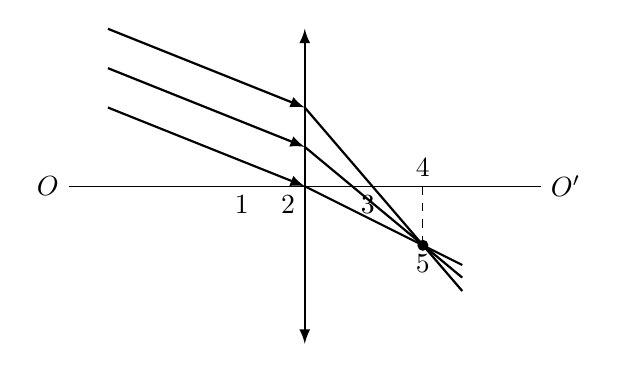
\begin{tikzpicture}[>=latex, scale=1]
    % Optik o'q
    \draw (0,0) -- (6,0) node[right] {$O'$};
    \node[left] at (0,0) {$O$};
    
    % Linza (yig'uvchi)
    \draw[thick, <->] (3,-2) -- (3,2);
    
    % Parallel nurlar (tushayotgan)
    \foreach \y in {0.5, 1, 1.5} {
        \draw[thick, ->] (0.5, \y+0.5) -- (3, \y-0.5);
    }
    
    % Singan nurlar (nuqtaga yig'iluvchi)
    \coordinate (F_prime) at (4.5, -1);
    \draw[thick] (3, 1) -- (5, -1.33);
    \draw[thick] (3, 0.5) -- (5, -1.16);
    \draw[thick] (3, 0) -- (5, -1);
    
    % Nuqtalar va raqamlar
    \node[below] at (2.2, 0) {1};
    \node[below left] at (3, 0) {2};
    \node[below] at (3.8, 0) {3};
    \node[above] at (4.5, 0) {4};
    \fill (4.5, -0.75) circle (2pt) node[below] {5};
    \draw[dashed] (4.5, 0) -- (4.5, -0.75);
\end{tikzpicture}

\begin{enumerate}[label=\Alph*)]
\item 1.
\item 2.
\item 3.
\item 4.
\end{enumerate}

\item Tasvirlangan linzalarning qaysilari yig‘uvchi?
\begin{enumerate}[label=\Alph*)]
\item 4, 5, 6.
\item 1, 2, 3.
\item 3, 4, 5.
\item 2, 3, 4.
\item 3, 5, 6.
\end{enumerate}

\item Nurning yo‘li qaysi rasmda to‘g‘ri ko‘rsatilgan?
\begin{enumerate}[label=\Alph*)]
\item A
\item B
\item C
\item D
\item E
\end{enumerate}

\item Uchta linzaning fokus masofalari $(F)$ teng bo‘lib, ular bir-biridan $F$ masofada joylashgan. A nur fokusdan o‘tib, birinchi linzaga tushadi. Nurning linzalar sistemasidan chiqqandan keyingi yo‘nalishini aniqlang.

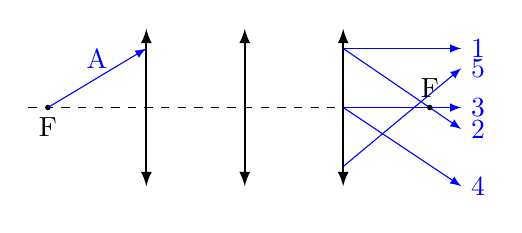
\begin{tikzpicture}[>=latex, scale=0.5]
    % Optik o'q
    \draw[dashed] (-4,0) -- (6,0);
    % Ikki linza
    \draw[thick, <->] (-1,-2) -- (-1,2);
    \draw[thick, <->] (1.5,-2) -- (1.5,2);
    \draw[thick, <->] (4,-2) -- (4,2);
    
    % Nur yo'li
    \fill (-3.5,0) circle (2pt) node[below] {F};
    \draw[blue, ->] (-3.5,0) -- (-1, 1.5) node[midway, above] {A};
    
    % Chiqayotgan nurlar
    \draw[blue,->] (4,1.5)--(7,1.5) node[right] {1};
    \draw[blue,->] (4,1.5)--(7,-0.55) node[right] {2};
    \draw[blue,->] (4,0)--(7,0) node[right] {3};
    \draw[blue,->] (4,0)--(7,-2) node[right] {4};
    \draw[blue,->] (4,-1.5)--(7,1) node[right] {5};
    
    
    \fill (6.2, 0) circle (2pt) node[above] {F};
\end{tikzpicture}

\begin{enumerate}[label=\Alph*)]
\item 4.
\item 5.
\item 3.
\item 2.
\item 1.
\end{enumerate}

\item Parallel nurlar dastasi fokus masofalari $F_1$ va $F_2$ bo‘lgan ikki yig‘uvchi linzadan o‘tib yana parallel ravishda tarqalishi uchun linzalarni qanday joylashtirish lozim?

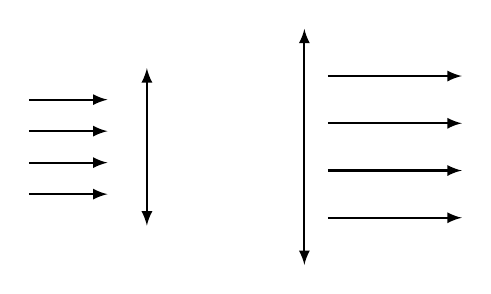
\begin{tikzpicture}[>=latex]
    % Linzalar
    \draw[thick, <->] (2,-1) -- (2,1);    % Birinchi (kichikroq) linza
    \draw[thick, <->] (4,-1.5) -- (4,1.5); % Ikkinchi (kattaroq) linza

    % Chap tomondagi nurlar
    \foreach \y in {-0.6, -0.2, 0.2, 0.6} {
        \draw[thick, ->] (0.5, \y) -- (1.5, \y);
    }


    % O'ng tomondagi nurlar
    \foreach \y in {-0.9, -0.3, 0.3, 0.9} {
        \draw[thick, ->] (4.3, \y) -- (6, \y);
    }
\end{tikzpicture}


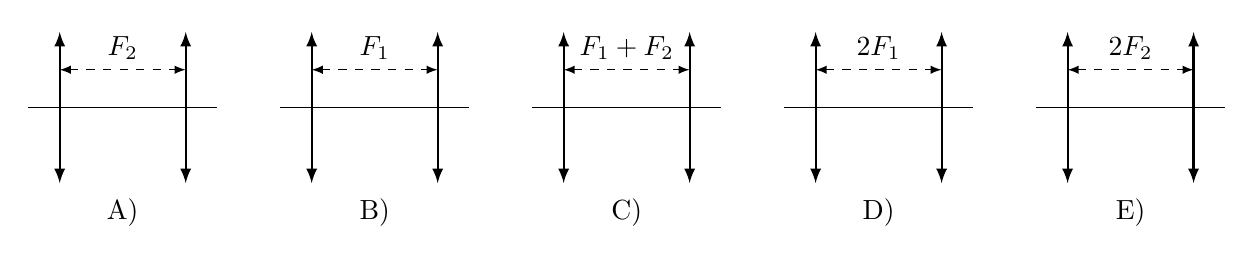
\begin{tikzpicture}[>=latex, scale=0.8]
    % A) holat
    \begin{scope}[shift={(0,0)}]
        \draw (-1.5,0) -- (1.5,0);
        \draw[thick, <->] (-1,-1.2) -- (-1,1.2);
        \draw[thick, <->] (1,-1.2) -- (1,1.2);
        \draw[dashed, <->] (-1,0.6) -- (1,0.6) node[midway, above] {$F_2$};
        \node[below] at (0,-1.3) {A)};
    \end{scope}

    % B) holat
    \begin{scope}[shift={(4,0)}]
        \draw (-1.5,0) -- (1.5,0);
        \draw[thick, <->] (-1,-1.2) -- (-1,1.2);
        \draw[thick, <->] (1,-1.2) -- (1,1.2);
        \draw[dashed, <->] (-1,0.6) -- (1,0.6) node[midway, above] {$F_1$};
        \node[below] at (0,-1.3) {B)};
    \end{scope}

    % C) holat
    \begin{scope}[shift={(8,0)}]
        \draw (-1.5,0) -- (1.5,0);
        \draw[thick, <->] (-1,-1.2) -- (-1,1.2);
        \draw[thick, <->] (1,-1.2) -- (1,1.2);
        \draw[dashed, <->] (-1,0.6) -- (1,0.6) node[midway, above] {$F_1+F_2$};
        \node[below] at (0,-1.3) {C)};
    \end{scope}

    % D) holat
    \begin{scope}[shift={(12,0)}]
        \draw (-1.5,0) -- (1.5,0);
        \draw[thick, <->] (-1,-1.2) -- (-1,1.2);
        \draw[thick, <->] (1,-1.2) -- (1,1.2);
        \draw[dashed, <->] (-1,0.6) -- (1,0.6) node[midway, above] {$2F_1$};
        \node[below] at (0,-1.3) {D)};
    \end{scope}

    % E) holat
    \begin{scope}[shift={(16,0)}]
        \draw (-1.5,0) -- (1.5,0);
        \draw[thick, <->] (-1,-1.2) -- (-1,1.2);
        \draw[thick, <->] (1,-1.2) -- (1,1.2);
        \draw[dashed, <->] (-1,0.6) -- (1,0.6) node[midway, above] {$2F_2$};
        \node[below] at (0,-1.3) {E)};
    \end{scope}
\end{tikzpicture}



\item Parallel nurlar 2 linzadan o‘tgach, parallelligicha qoldi. Agar bu linzalarning ikkalasi ham yig‘uvchi bo‘lsa, ular qanday joylashgan?
\begin{enumerate}[label=\Alph*)]
\item bir-biriga bevosita tegib turibdi.
\item linzalar orasidagi masofa fokus masofalari yig‘indisidan ancha katta.
\item birinchi linzaning orqa fokal tekisligi ikkinchi linzaning oldingi fokal tekisligi bilan mos tushadi.
\item javob fokus masofalari nisbatiga bog‘liq.
\item bunday bo‘lishi mumkin emas.
\end{enumerate}

\item Fokus masofasi $F$ bo‘lgan yupqa sochuvchi linzaga bosh optik o‘qiga nisbatan $\alpha$ burchak ostida nur tushmoqda. Bu nur linzaning orqasida joylashgan shaffof ekranni bosh optik o‘qdan qanday balandlikda (cm) kesib o‘tadi?

\begin{tikzpicture}[scale=0.8]
    % Optik o'q
    \draw (-3,0) -- (4,0);
    
    % Sochiluvchi linza belgisi
    \draw[thick, >-<] (0,-2) -- (0,2);
    
    % Fokus nuqtalari
    \fill (-1.5,0) circle (2pt) node[below] {F};
    \fill (1.5,0) circle (2pt) node[below] {F};
    
    % E ekrani
    \draw[thick] (2.25, 0) -- (2.25, 1.8) node[right] {E};
    \node[below] at (2.25, 0) {3F/2};
    
    % Nur yo'li
    \draw[thick, ->,red] (-1.5, 2.5) -- (0, 1.2); % Kelayotgan nur
    \draw[dashed] (0, 1.2) -- (3, -1.25); % Nur yo'nalishi (fokusga qarab)
    
    % Burchak alfa
    \draw (1, 0) arc (180:143:0.5);
    \node at (0.7, 0.3) {\Large $\alpha$};
\end{tikzpicture}

\begin{enumerate}[label=\Alph*)]
\item $0$.
\item $F\cos\alpha$.
\item $F\sin\alpha$.
\item $F\cdot tg \alpha$.
\item $F/2$.
\end{enumerate}

\item Ushbu rasmda nurning ikkita qavariq linzalardan o‘tib ketish jarayoni keltirilgan. Rasmga foydalanib, linzalarning fokus masofalari nisbatini $F_1/F_2$ ni toping.

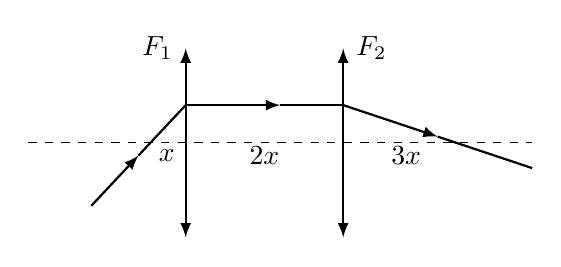
\begin{tikzpicture}[>=latex,scale=0.8]
    % Optik o'q
    \draw[dashed] (-1,0) -- (7,0);
    
    % Linzalar
    \draw[thick, <->] (1.5,-1.5) -- (1.5,1.5) node[left=1pt] {$F_1$};
    \draw[thick, <->] (4,-1.5) -- (4,1.5) node[right=1pt] {$F_2$};
    
    % Nur yo'li
    \draw[thick, ->] (0,-1) -- (0.75, -0.2); 
    \draw[thick] (0.75, -0.2) -- (1.5, 0.6); % Linzagacha
    \draw[thick, ->] (1.5, 0.6) -- (3, 0.6);  % Parallel qism
    \draw[thick] (3, 0.6) -- (4, 0.6);
    \draw[thick, ->] (4, 0.6) -- (5.5, 0.1);  % Chiquvchi nur
    \draw[thick] (5.5, 0.1) -- (7, -0.4);
    
    % Masofa belgilari
    \node at (1.2, -0.2) {$x$};
    \node at (2.75, -0.2) {$2x$};
    \node at (5, -0.2) {$3x$};
\end{tikzpicture}

\begin{enumerate}[label=\Alph*)]
\item $1/2$
\item $2/3$
\item $1/3$
\item $1/6$
\item $3/4$
\end{enumerate}

\item Ushbu rasmdagi 1 nur qavariq linzadan o‘tgach qaysi nuqtadan o‘tadi? $F$ — linzaning fokus masofasi.

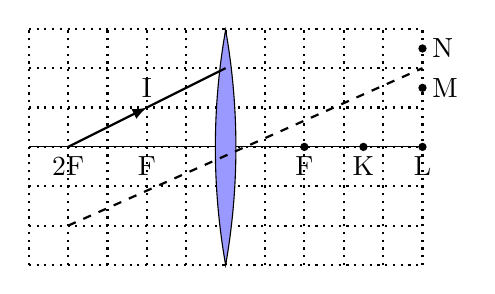
\begin{tikzpicture}[scale=0.5]
    % Grid
    \draw[step=1, dotted, thick] (-5,-3) grid (5,3);
    \draw (-5,0) -- (5,0);
    
    % Linza
    \filldraw[fill=blue!40] (0,-3) arc (-10:10:17.2) arc (170:190:17.2) -- cycle;
    
    % Nuqtalar (chapda)
    \node[below] at (-4,0) {2F};
    \node[below] at (-2,0) {F};
    
    % Nuqtalar (o'ngda)
    \fill (2,0) circle (3pt) node[below] {F};
    \fill (3.5,0) circle (3pt) node[below] {K};
    \fill (5,0) circle (3pt) node[below] {L};
    \fill (5,1.5) circle (3pt) node[right] {M};
    \fill (5,2.5) circle (3pt) node[right] {N};
    
    % Nur I
    \draw[thick, ->, >=latex] (-4,0) -- (-2,1) node[above] {I};
    \draw[thick] (-2,1) -- (0,2);
    \draw[dashed, thick] (-4,-2) -- (5,2);
\end{tikzpicture}

\begin{enumerate}[label=\Alph*)]
\item F.
\item K.
\item L.
\item M.
\item N.
\end{enumerate}

\item Ushbu rasmdagi 1 nur qavariq linzadan o‘tgach qaysi nuqtadan o‘tadi? $F$ — linzaning fokus masofasi.

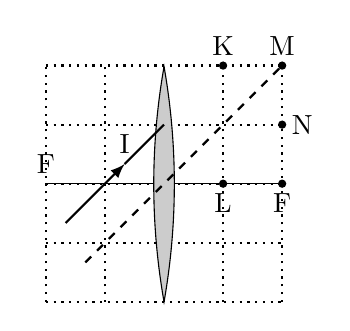
\begin{tikzpicture}[scale=0.5]
    % Grid
    \draw[step=1.5, dotted, thick] (-3,-3) grid (3,3);
    \draw (-3,0) -- (3,0);
    
    % Linza
    \filldraw[fill=gray!40] (0,-3) arc (-10:10:17.2) arc (170:190:17.2) -- cycle;
    
    % Nuqtalar
    \fill (3,0) circle (3pt) node[below] {F};
    \fill (1.5,0) circle (3pt) node[below] {L};
    \node[above] at (-3,0) {F};
    \fill (1.5,3) circle (3pt) node[above] {K};
    \fill (3,3) circle (3pt) node[above] {M};
    \fill (3,1.5) circle (3pt) node[right] {N};
    
    % Nur I
    \draw[thick, ->, >=latex] (-2.5,-1) -- (-1,0.5) node[above] {I};
    \draw[thick] (-1,0.5) -- (0,1.5);
    \draw[dashed, thick] (-2,-2) -- (3,3);
\end{tikzpicture}

\begin{enumerate}[label=\Alph*)]
\item F.
\item K.
\item L.
\item M.
\item N.
\end{enumerate}

\item Ushbu rasmdagi 1 nur qavariq linzadan o‘tgach qaysi nuqtadan o‘tadi? $F$ — linzaning fokus masofasi.

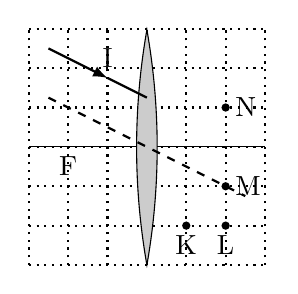
\begin{tikzpicture}[scale=0.5]
    % Grid
    \draw[step=1, dotted, thick] (-3,-3) grid (3,3);
    \draw (-3,0) -- (3,0);
    
    % Linza
    \filldraw[fill=gray!40] (0,-3) arc (-10:10:17.2) arc (170:190:17.2) -- cycle;
    
    % Nuqtalar
    \node[below] at (-2,0) {F};
    \fill (1,-2) circle (3pt) node[below] {K};
    \fill (2,-2) circle (3pt) node[below] {L};
    \fill (2,-1) circle (3pt) node[right] {M};
    \fill (2,1) circle (3pt) node[right] {N};
    
    % Nur I
    \draw[thick, ->, >=latex] (-2.5,2.5) -- (-1,1.75) node[above] {I};
    \draw[thick] (-1,1.75) -- (0,1.25);
    \draw[dashed, thick] (-2.5,1.25) -- (2.5,-1.25);
\end{tikzpicture}


\begin{enumerate}[label=\Alph*)]
\item F.
\item K.
\item L.
\item M.
\item N.
\end{enumerate}

\item Rasmda ko‘rsatilgan qaysi biri linzaning fokusi, qaysi biri optik markazidir?

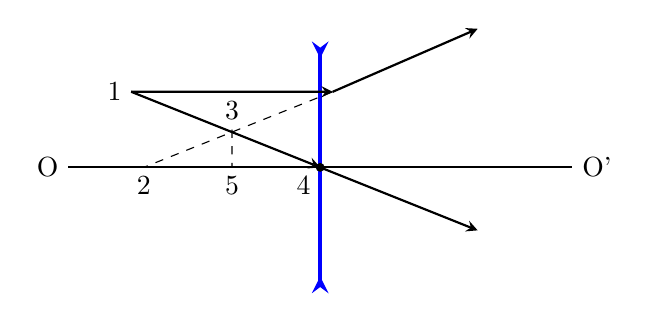
\begin{tikzpicture}[>=stealth,scale=0.8]
    % Optik o'q
    \draw[thick] (-4,0) -- (4,0) node[right] {O'};
    \node[left] at (-4,0) {O};
    
    \draw[ultra thick, blue,>-<] (0,-2)--(0,2);
    
    
    % Nurlar va nuqtalar
    \coordinate (P1) at (-3, 1.2); \node[left] at (P1) {1};
    \coordinate (P2) at (-2.8, 0); \node[below] at (P2) {2};
    \coordinate (P4) at (0, 0); \fill (P4) circle (2pt) node[below left] {4};
    
    % Nur 1 dan parallel
    \draw[thick, ->] (P1) -- (0.2, 1.2);
    \draw[thick, ->] (0.2, 1.2) -- (2.5, 2.2);
    \draw[dashed] (0.2, 1.2) -- (P2); % Virtual nur
    
    % Nur 1 dan markaz orqali
    \draw[thick, ->] (P1) -- (P4);
    \draw[thick, ->] (P4) -- (2.5, -1);
    
    % Nuqta 3 va 5
    \coordinate (P3) at (-1.4, 0.6); \node[above] at (P3) {3};
    \draw[dashed] (P3) -- (-1.4, 0) node[below] {5};
\end{tikzpicture}

\begin{enumerate}[label=\Alph*)]
\item 4, 5.
\item 3, 5.
\item 2, 3.
\item 1, 4.
\item 2, 4.
\end{enumerate}

\item Quyidagi uchta holatdan qaysi birida nurning sochuvchi linzadan o‘tish jarayoni to‘g‘ri tasvirlangan?

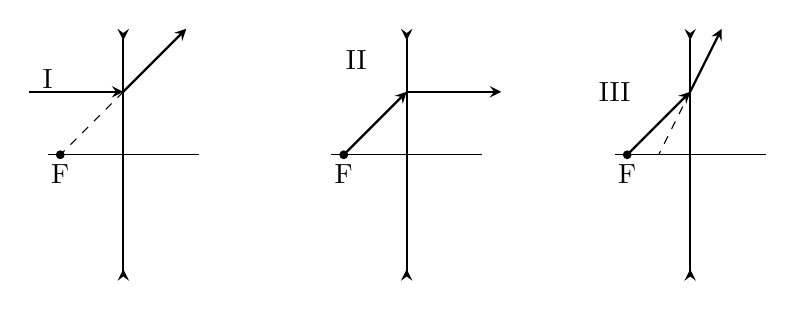
\begin{tikzpicture}[>=stealth, scale=0.8]
    % I-holat: Parallel keluvchi nur
    \begin{scope}[shift={(0,0)}]
        \draw (-1.2,0) -- (1.2,0);
        \draw[thick, >-<] (0,-2) -- (0,2);
        \fill (-1,0) circle (2pt) node[below] {F};
        \draw[thick, ->] (-1.5,1) -- (0,1);
        \draw[thick, ->] (0,1) -- (1,2);
        \draw[dashed] (0,1) -- (-1,0);
        \node at (-1.2,1.2) {I};
    \end{scope}
    
    % II-holat: Fokusga yo'nalgan nur
    \begin{scope}[shift={(4.5,0)}]
        \draw (-1.2,0) -- (1.2,0);
        \draw[thick, >-<] (0,-2) -- (0,2);
        \fill (-1,0) circle (2pt) node[below] {F};
        \draw[thick, <-] (0,1) -- (-1,0); % Fokusdan chiqqandek yo'nalish
        \draw[thick, ->] (0,1) -- (1.5,1);
        \node at (-0.8,1.5) {II};
    \end{scope}
    
    % III-holat: Fokus orqali o'tuvchi nur
    \begin{scope}[shift={(9,0)}]
        \draw (-1.2,0) -- (1.2,0);
        \draw[thick, >-<] (0,-2) -- (0,2);
        \fill (-1,0) circle (2pt) node[below] {F};
        \draw[thick, <-] (0,1) -- (-1,0);
        \draw[thick, ->] (0,1) -- (0.5,2);
        \draw[dashed] (0,1) -- (-0.5,0);
        \node at (-1.2,1) {III};
    \end{scope}
\end{tikzpicture}

\begin{enumerate}[label=\Alph*)]
\item I.
\item II.
\item III.
\item I va II.
\item II va III.
\end{enumerate}

\item Ushbu rasmda nurning linzadan o‘tish jarayoni keltirilgan. Qaysi nuqta linzaning fokusi hisoblanadi?

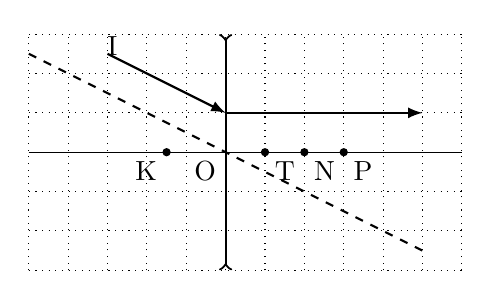
\begin{tikzpicture}[scale=0.5]
    % Grid
    \draw[step=1, dotted] (-5,-3) grid (6,3);
    \draw (-5,0) -- (6,0);
    
    % Sochiluvchi linza
    \draw[thick, >-<] (0,-3) -- (0,3);
    
    % Nuqtalar
    \fill (-1.5,0) circle (3pt) node[below left] {K};
    \node[below left] at (0,0) {O};
    \fill (1,0) circle (3pt) node[below right] {T};
    \fill (2,0) circle (3pt) node[below right] {N};
    \fill (3,0) circle (3pt) node[below right] {P};
    
    % Nur I
    \draw[thick, ->, >=latex] (-3,2.5) -- (0,1);
    \node[above left] at (-2.5,2.2) {I};
    \draw[thick, ->, >=latex] (0,1) -- (5,1);
    
    % Punktir chiziq
    \draw[dashed, thick] (-5,2.5) -- (5,-2.5);
\end{tikzpicture}

\begin{enumerate}[label=\Alph*)]
\item K.
\item T.
\item N.
\item P.
\end{enumerate}

\item Ushbu rasmda nur botiq linzadan o‘tgach qaysi yo‘nalishda ketadi? $F$ — linzaning fokus masofasi.

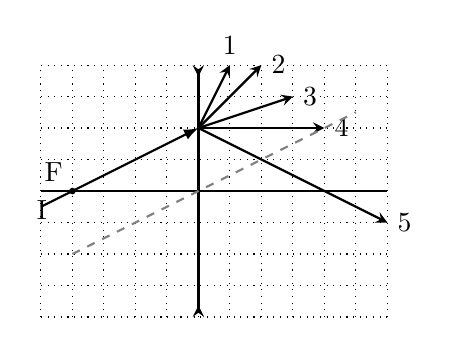
\begin{tikzpicture}[>=stealth,scale=0.4]
    % Grid
    \draw[step=1, dotted] (-5,-4) grid (6,4);
    \draw (-5,0) -- (6,0);
    
    % Sochiluvchi linza
    \draw[thick, >-<] (0,-4) -- (0,4);
    
    % Fokus F va nur I
    \fill (-4,0) circle (3pt) node[above left] {F};
    \node[below left] at (-4.5,0) {I};
    \draw[thick, ->, >=latex] (-5,-0.5) -- (0,2);
    
    % Chiqayotgan nurlar
    \draw[thick, ->] (0,2) -- (1,4) node[above] {1};
    \draw[thick, ->] (0,2) -- (2,4) node[right] {2};
    \draw[thick, ->] (0,2) -- (3,3) node[right] {3};
    \draw[thick, ->] (0,2) -- (4,2) node[right] {4};
    \draw[thick, ->] (0,2) -- (6,-1) node[right] {5};
    
    % Punktir yo'nalish
    \draw[dashed, thick,gray] (-4,-2) -- (5,2.5);
\end{tikzpicture}

\begin{enumerate}[label=\Alph*)]
\item 1.
\item 2.
\item 3.
\item 4.
\item 5.
\end{enumerate}

\item Ushbu rasmda nurning ikkita botiq linzalardan o‘tib ketish jarayoni keltirilgan. Undan foydalanib, linzalarning fokus masofalari bir xil bo‘lsa, qo‘shni nuqtalar orasidagi masofalar nisbati $F_1/F_2$ ni toping.

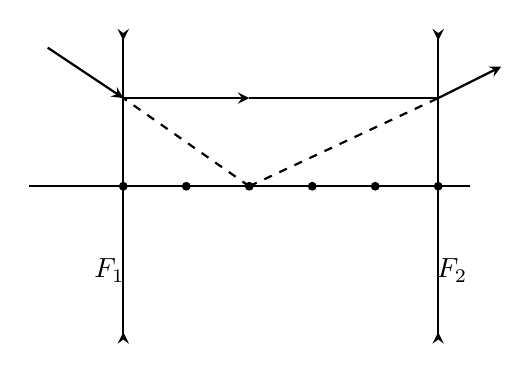
\begin{tikzpicture}[>=stealth, scale=0.8]
    % Optik o'q (Horizontal chiziq)
    \draw[thick] (-3.5,0) -- (3.5,0);
    
    % Birinchi sochiluvchi linza (F1)
    \draw[thick, >-<] (-2,-2.5) -- (-2,2.5);
    \node[left=5pt, below] at (-2, -1) {$F_1$};
    
    % Ikkinchi sochiluvchi linza (F2)
    \draw[thick, >-<] (3,-2.5) -- (3,2.5);
    \node[right=5pt, below] at (3, -1) {$F_2$};
    
    % Optik o'qdagi nuqtalar
    \fill (-2,0) circle (2pt); % F1 markazi
    \fill (-1,0) circle (2pt);
    \fill (0,0) circle (2pt);  % Markaziy nuqta
    \fill (1,0) circle (2pt);
    \fill (2,0) circle (2pt);
    \fill (3,0) circle (2pt);% F2 markazi
    
    % Nurlar yo'li (Haqiqiy nurlar - qalin chiziqlar)
    % 1. Kiruvchi nur
    \draw[thick, ->] (-3.2, 2.2) -- (-2, 1.4);
    % 2. Linzalar orasidagi gorizontal nur
    \draw[thick, ->] (-2, 1.4) -- (0, 1.4);
    \draw[thick] (0, 1.4) -- (3, 1.4);
    % 3. Chiquvchi nur
    \draw[thick, ->] (3, 1.4) -- (4,1.9);
    
    % Virtual nurlar (Punktir chiziqlar)
    % Markaziy nuqtadan (0,0) linzalarning sinish nuqtalarigacha
    \draw[dashed, thick] (0,0) -- (-2, 1.4);
    \draw[dashed, thick] (0,0) -- (3, 1.4);
    
\end{tikzpicture}

\begin{enumerate}[label=\Alph*)]
\item $1/2$
\item $2/3$
\item $1/3$
\item $3/2$
\item $3/4$
\end{enumerate}

\end{enumerate}
\begin{center}
\begin{tabular}{|c|c|c|c|c|c|c|c|c|c|}
\hline
1e & 2d & 3d & 4a & 5c & 6c & 7d & 8c & 9c & 10d\\
\hline
11d & 12e & 13d & 14d & 15b & 16b & & & & \\
\hline
\end{tabular}
\end{center}


